\documentclass[tikz,border=7pt]{standalone}
\usepackage[T1]{fontenc}
\usepackage[utf8]{inputenc}
\usetikzlibrary{positioning,arrows.meta}
\begin{document}
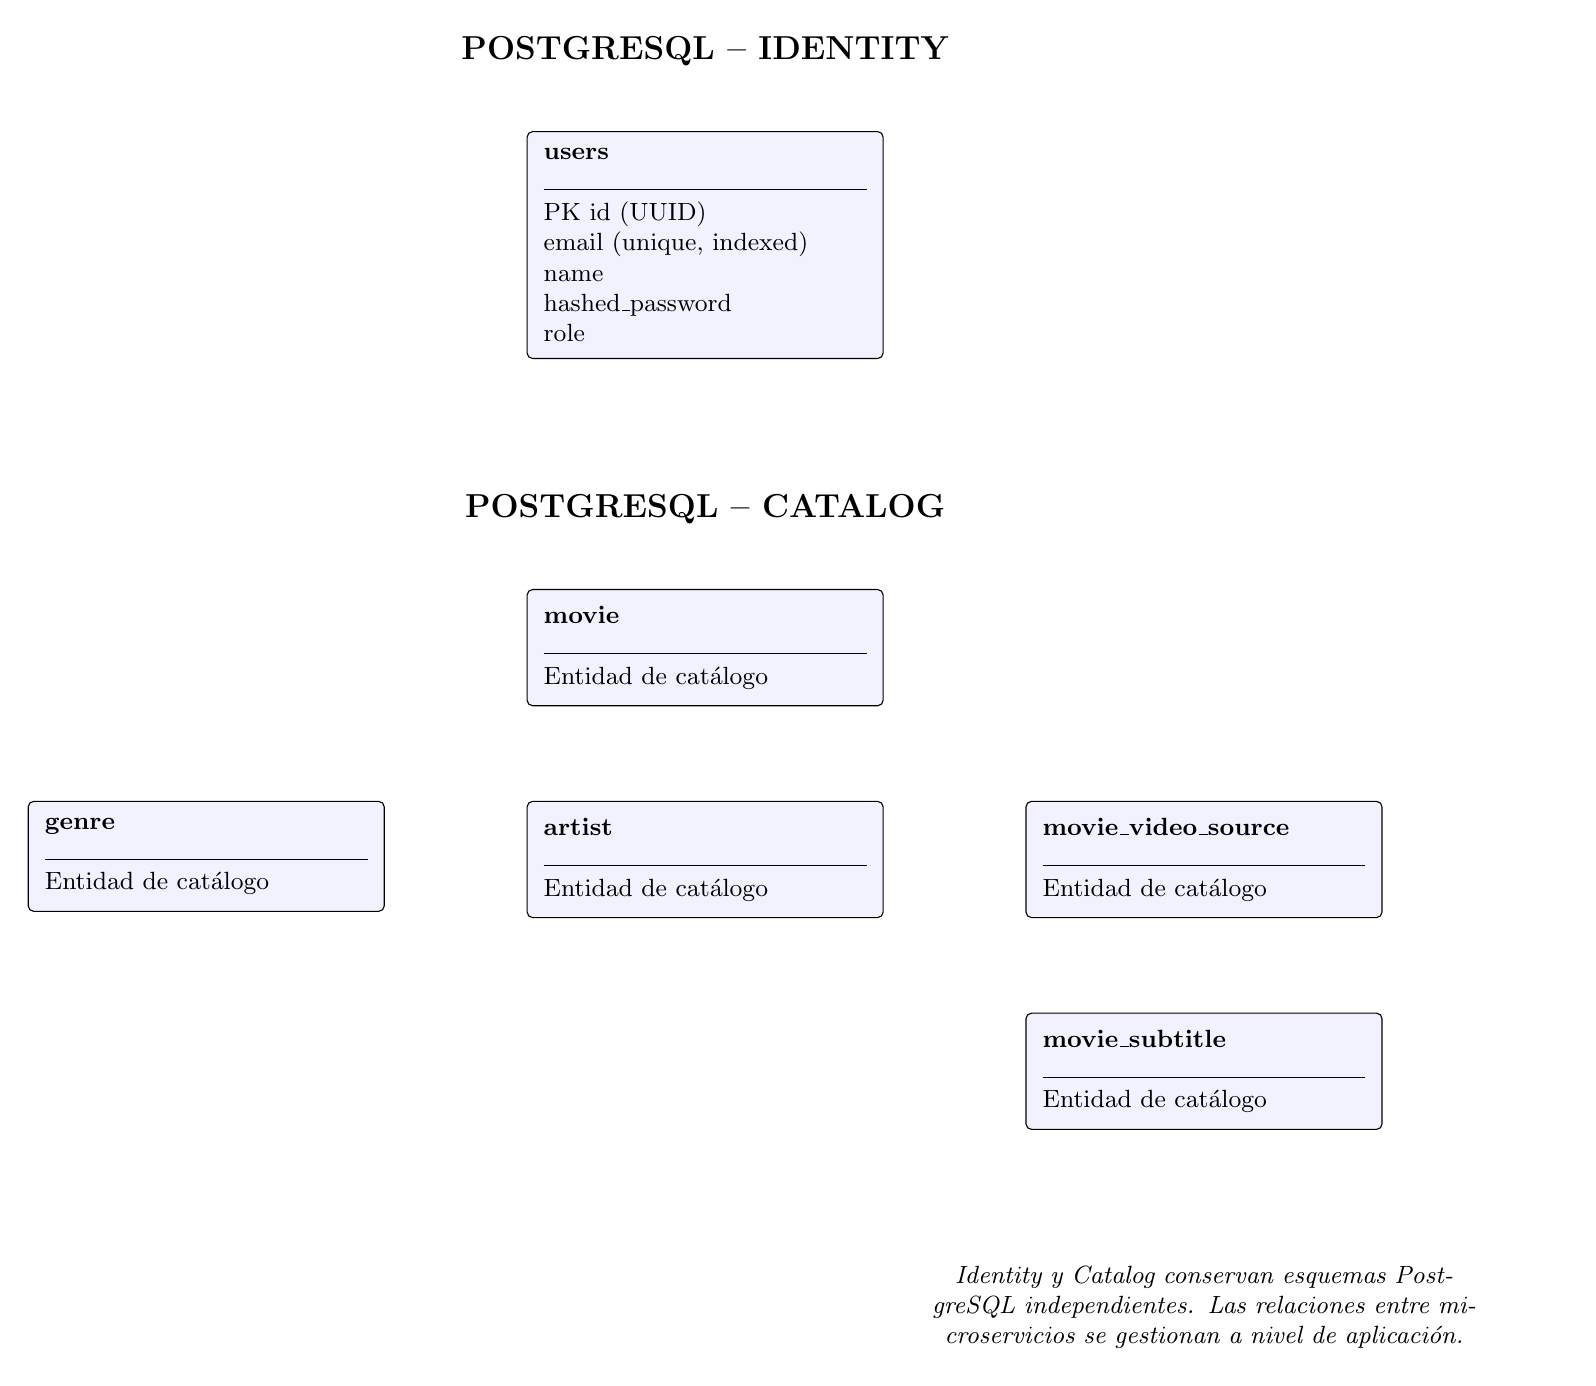
\begin{tikzpicture}[font=\small, entity/.style={draw, rounded corners=2pt, align=left, text width=4.1cm, inner sep=6pt, fill=blue!5}, heading/.style={font=\bfseries\large}, note/.style={align=center, text width=9cm, font=\small\itshape}]
\node[heading] (identitytitle) {POSTGRESQL -- IDENTITY};
\node[entity, below=7mm of identitytitle] (users) {\textbf{users}\\\rule{4.1cm}{0.3pt}\\PK id (UUID)\\email (unique, indexed)\\name\\hashed\_password\\role};
\node[heading, below=16mm of users] (catalogtitle) {POSTGRESQL -- CATALOG};
\node[entity, below=7mm of catalogtitle] (movie) {\textbf{movie}\\\rule{4.1cm}{0.3pt}\\Entidad de catálogo};
\node[entity, below left=12mm and 18mm of movie] (genre) {\textbf{genre}\\\rule{4.1cm}{0.3pt}\\Entidad de catálogo};
\node[entity, below=12mm of movie] (artist) {\textbf{artist}\\\rule{4.1cm}{0.3pt}\\Entidad de catálogo};
\node[entity, below right=12mm and 18mm of movie] (video) {\textbf{movie\_video\_source}\\\rule{4.1cm}{0.3pt}\\Entidad de catálogo};
\node[entity, below=12mm of video] (subtitle) {\textbf{movie\_subtitle}\\\rule{4.1cm}{0.3pt}\\Entidad de catálogo};
\node[note, below=16mm of subtitle] {Identity y Catalog conservan esquemas PostgreSQL independientes. Las relaciones entre microservicios se gestionan a nivel de aplicación.};
\end{tikzpicture}
\end{document}
